\documentclass[../Main.tex]{subfiles}
\begin{document}

\section*{Introduction}
\addcontentsline{toc}{section}{Introduction}

This chapter establishes the theoretical bedrock upon which our experimental work is built. It provides a comprehensive overview of Reinforcement Learning, starting from the foundational principles of single-agent systems and progressively building toward the complex multi-agent paradigms relevant to this project.

The discussion begins by defining the core concepts of Reinforcement Learning, including the Markov Decision Process, value functions, and the Bellman equations. It then surveys the classical and modern algorithms designed to solve these problems, charting a path from Dynamic Programming to the landmark Deep Q-Learning algorithm. Finally, the chapter transitions to the multi-agent domain, detailing the challenges of coordination and introducing the QMIX algorithm as a key point of reference for our own research.

\section{Reinforcement Learning (RL): General Concept}

Reinforcement Learning (RL) is a fundamental framework in machine learning where an agent learns how to act within an environment by trial and error \cite{sutton2018reinforcement}. The agent interacts with the environment in discrete time steps, taking actions and receiving feedback in the form of numerical rewards. Over time, the goal of the agent is to learn a strategy that maximizes the cumulative reward it collects.

At a high level, the agent perceives the current situation, often referred to as the \emph{state}, and selects an \emph{action} according to a decision-making rule called a \emph{policy}. The environment then transitions to a new state and emits a \emph{reward}, reflecting the quality or usefulness of the chosen action. This interaction forms a feedback loop, through which the agent gradually learns an improved policy based on its past experiences.

\begin{figure}[H]
    \centering
    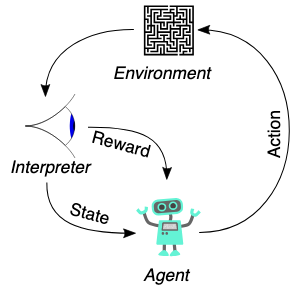
\includegraphics[width=0.35\textwidth]{img/rl-diagram.png}
    \caption{Illustrative example of how RL works: the agent-environment interaction loop.}
    \label{fig:rl-loop}
\end{figure}

Figure~\ref{fig:rl-loop} summarizes this loop. The agent observes the state of the environment, takes an action, and in return receives a new state and a reward. The feedback from the environment allows the agent to assess the effectiveness of its actions and adapt its strategy accordingly.

\begin{figure}[H]
    \centering
    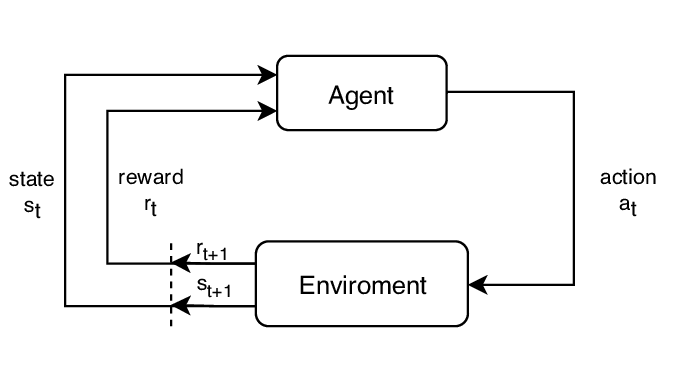
\includegraphics[width=0.75\textwidth]{img/rl-summary.png}
    \caption{Standard reinforcement learning interaction loop. At each timestep \(t\), the agent observes state \(s_t\), takes action \(a_t\), and receives a reward \(r_t\) and next state \(s_{t+1}\) from the environment.}
    \label{fig:rl-loop-precise}
\end{figure}

Figure~\ref{fig:rl-loop-precise} provides a more precise view of the agent-environment interaction in reinforcement learning. At each timestep \(t\), the agent observes the current state \(s_t\) and selects an action \(a_t\) according to its policy. This action is sent to the environment, which responds by producing the next state \(s_{t+1}\) and a scalar reward \(r_{t+1}\). These two elements — reward and next state — serve as feedback to guide the agent’s learning process.

This feedback loop continues over time, and the agent’s objective is to optimize its behavior to maximize the cumulative sum of future rewards. Note that the reward \(r_{t+1}\) corresponds to the outcome of the action \(a_t\) taken from state \(s_t\), reflecting the delayed nature of feedback in RL systems.

The basic reinforcement learning terms will be formally defined and explored in detail in the following sections. At this stage, the goal is to establish an intuitive understanding of the learning paradigm: the agent uses environmental feedback to adapt its behavior over time, seeking to improve its long-term performance through experience.

Compared to other common machine learning paradigms, Reinforcement Learning is distinct in both its structure and objectives. Unlike supervised learning, which relies on labeled datasets and direct feedback, RL is based on interaction and delayed reward signals. The table below highlights the key differences:

\begin{table}[H]
\centering
\small
\renewcommand{\arraystretch}{1.2}
\begin{tabular}{|p{3.2cm}|p{5cm}|p{5cm}|}
    \hline
    \textbf{Aspect} & \textbf{Supervised Learning} & \textbf{Reinforcement Learning} \\
    \hline
    Data Labeling & Requires labeled input-output pairs & No labels; relies on scalar reward signals \\
    \hline
    Feedback Type & Immediate and direct (per sample) & Delayed and sparse, based on action outcomes \\
    \hline
    Objective & Minimize prediction error on known targets & Maximize expected long-term cumulative reward \\
    \hline
    Interaction Type & One-shot on fixed dataset & Sequential decision-making with environment interaction \\
    \hline
    Typical Applications & Classification, regression tasks & Game playing, control, robotics, online decision-making \\
    \hline
\end{tabular}
\caption{Comparison between supervised learning and reinforcement learning.}
\label{tab:supervised-vs-rl}
\end{table}


Reinforcement Learning has been successfully applied in a wide range of domains, including robotics, game playing, recommendation systems, and autonomous control. Its strength lies in its ability to learn optimal behavior in complex, uncertain environments without requiring explicit supervision.


\section{Markov Decision Processes (MDPs)}

A Markov Decision Process (MDP) is a mathematical framework used for modeling decision-making problems where outcomes are partly random and partly under the control of a decision-maker \cite{bellman1957dynamic}. An MDP is defined by the following components:

\begin{figure}[H]
    \centering
    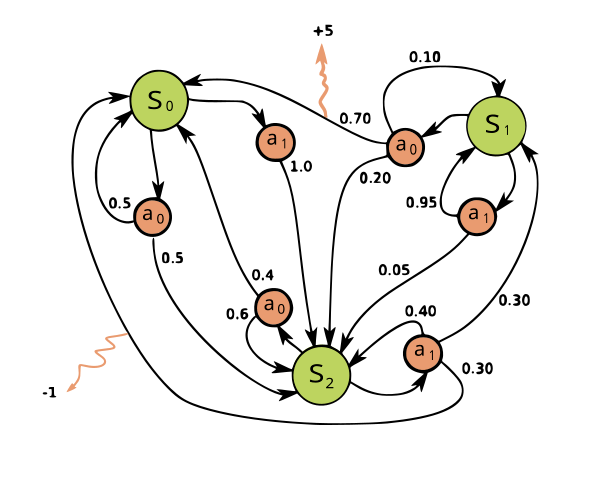
\includegraphics[width=0.7\textwidth]{img/mdp.png}
    \caption{Visualization of a simple MDP.}
\end{figure}

\begin{itemize}
    \item \textbf{State Space} ($S$): A finite set of states representing all possible situations in which an agent can be.
    \item \textbf{Action Space} ($A$): A finite set of actions available to the agent.
    \item \textbf{Transition Function} ($P$): A function $P(s'|s,a)$ representing the probability of transitioning to state $s'$ from state $s$ after taking action $a$.
    \item \textbf{Reward Function} ($R$): A function $R(s,a)$ representing the immediate reward received after taking action $a$ in state $s$.
    \item \textbf{Discount Factor} ($\gamma$): A factor $0 \leq \gamma \leq 1$ that represents the present value of future rewards.
\end{itemize}

\textbf{The Markov Property}

The Markov Property is a fundamental characteristic of MDPs, stating that the future state depends only on the current state and action, not on the sequence of events that preceded it. Formally, an MDP satisfies the Markov Property if:

\begin{equation}
    P(s_{t+1} | s_t, a_t, s_{t-1}, a_{t-1}, \ldots, s_0, a_0) = P(s_{t+1} | s_t, a_t)
\end{equation}

This implies that the state $s_t$ captures all relevant information from the history of the process needed to predict the next state $s_{t+1}$.

% \section{Partially Observable Markov Decision Processes (POMDPs)}

% A Partially Observable Markov Decision Process (POMDP) extends MDPs to situations where the agent does not have full observability of the state space or is uncertain about its observations \cite{cassandra1994acting}. A POMDP includes all MDP components plus:

% \begin{itemize}
%     \item \textbf{Observation Space} ($O$): A set of observations that the agent can receive.
%     \item \textbf{Observation Function} ($Z(o|s,a)$): A function representing the probability of observing $o$ given the state $s$ and action $a$.
% \end{itemize}

% \begin{figure}[H]
%     \centering
%     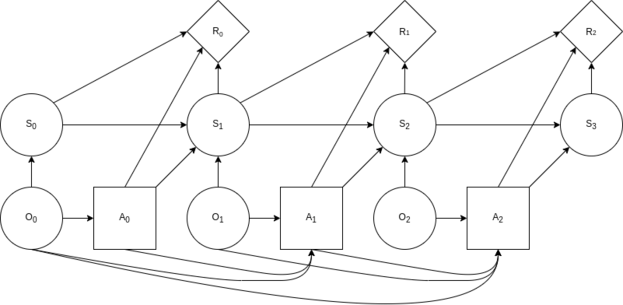
\includegraphics[width=1\linewidth]{img/pomdp.png}
%     \caption{Visualization of a simple POMDP}
%     \label{fig:pomdp-diagram}
% \end{figure}

% \textbf{Analogy:} A POMDP is to an MDP what a Hidden Markov Model is to a Markov Chain.

% \begin{table}[h]
%     \centering
%     \begin{tabular}{|l|c|c|}
%     \multicolumn{1}{c}{} & \multicolumn{2}{c}{\textbf{Control over state transitions?}} \\ \cline{2-3}
%     \multicolumn{1}{c|}{} & \textbf{NO} & \textbf{YES} \\
%     \hline
%     \textbf{States completely observable?} & Markov Chain & Markov Decision Process \\
%     \hline
%     \textbf{States partially observable?} & Hidden Markov Model & POMDP \\
%     \hline
%     \end{tabular}
%     \caption{Relationship between different stochastic process models}
% \end{table}

% POMDPs provide a more realistic framework for many real-world problems where the agent must make decisions based on incomplete or uncertain information.
% 
\section{Partially Observable Markov Decision Processes (POMDPs)}

In many real-world problems, an agent cannot perceive the environment's true state directly. A \textbf{Partially Observable Markov Decision Process (POMDP)} extends the MDP framework to model this uncertainty \cite{cassandra1994acting}. A POMDP includes all components of an MDP, plus two additions:
\begin{itemize}
    \item \textbf{Observation Space} ($\Omega$): A set of observations that the agent can receive.
    \item \textbf{Observation Function} ($O$): A function, often written as $O(o|s',a)$, representing the probability of receiving observation $o$ after taking action $a$ and landing in state $s'$.
\end{itemize}

Figure~\ref{fig:pomdp-diagram} provides a graphical model of the POMDP interaction loop. At each step, the agent is in a true underlying state \(S_t\) which it cannot see. Instead, it receives a correlated observation \(O_t\). Based on this observation, the agent selects an action \(A_t\). This action causes the environment to transition to a new hidden state \(S_{t+1}\) and emit a reward \(R_t\). This dependency structure highlights the core challenge of a POMDP: the agent must make decisions based on incomplete information, often by maintaining a belief or probability distribution over the possible true states.

\begin{figure}[H]
    \centering
    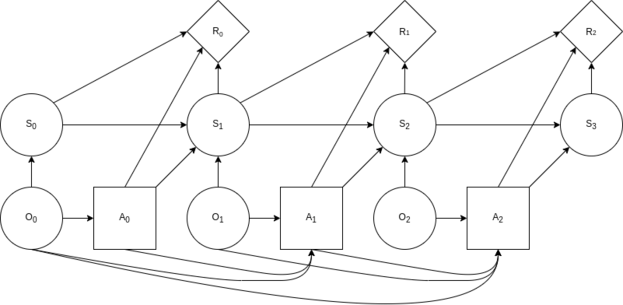
\includegraphics[width=1\linewidth]{img/pomdp.png}
    \caption{A graphical model of a Partially Observable Markov Decision Process. The agent's actions are based on observations, which are imperfect reflections of the true underlying state.}
    \label{fig:pomdp-diagram}
\end{figure}

To better understand where the POMDP framework fits within the landscape of stochastic models, Table~\ref{tab:pomdp_context} compares it to related processes. The table is organized along two axes: whether the state is fully observable and whether the agent has control over state transitions. A POMDP is the most general of these four models, applicable to situations where the agent has control but only partial observability. This makes it a realistic and powerful framework for a wide range of real-world problems.

\begin{table}[H]
    \centering
    \begin{tabular}{|l|c|c|}
    \multicolumn{1}{c}{} & \multicolumn{2}{c}{\textbf{Control over state transitions?}} \\ \cline{2-3}
    \multicolumn{1}{c|}{} & \textbf{NO} & \textbf{YES} \\
    \hline
    \textbf{States completely observable?} & Markov Chain & Markov Decision Process \\
    \hline
    \textbf{States partially observable?} & Hidden Markov Model & POMDP \\
    \hline
    \end{tabular}
    \caption{Relationship between different stochastic process models, contextualizing the Partially Observable Markov Decision Process.}
    \label{tab:pomdp_context}
\end{table}
% 

\section{Policies and Value Functions}

\subsection{Policy}

A policy ($\pi$) defines the behavior of the agent, specifying the action to be taken in each state. It can be deterministic or stochastic:

\begin{itemize}
    \item \textbf{Deterministic Policy} ($\pi(s)$): A function that maps each state to a specific action.
    \item \textbf{Stochastic Policy} ($\pi(a|s)$): A function that maps each state to a probability distribution over actions.
\end{itemize}

\subsection{Return and Discounting}

In reinforcement learning, an agent interacts with an environment by taking actions, observing states, and receiving rewards. The reward $r_t = R(s_t, a_t)$ is a scalar signal received from the environment after the agent performs an action in a given state.

However, making decisions based only on immediate reward is shortsighted. Instead, agents aim to maximize long-term performance through the concept of \textbf{return}. The return $G_t$ is the total accumulated reward from time $t$ onward:

\begin{equation}
    G_t = r_t + \gamma r_{t+1} + \gamma^2 r_{t+2} + \dots = \sum_{k=0}^{\infty} \gamma^k r_{t+k}
\end{equation}

The discount factor $\gamma \in [0, 1)$ determines the importance of future rewards: values close to 0 make the agent short-sighted, while values near 1 make it far-sighted.

\subsection{Value Functions}

Value functions quantify how good it is to be in a certain state or take a certain action under a specific policy $\pi$. They estimate the expected return the agent can accumulate \cite{sutton2018reinforcement}.

\subsubsection{State-Value Function:}
The state-value function $V^{\pi}(s)$ represents the expected cumulative reward when starting in state $s$ and following policy $\pi$:

\begin{equation}
    V^{\pi}(s) = \mathbb{E}_\pi\left[ G_t \mid s_t = s \right] = \mathbb{E}_\pi\left[\sum_{k=0}^{\infty} \gamma^k r_{t+k} \,\bigg|\, s_t = s\right]
\end{equation}

\subsubsection{Action-Value Function (Q-function):}
The action-value function $Q^{\pi}(s, a)$ evaluates the expected return starting from state $s$, taking action $a$, and then following policy $\pi$:

\begin{equation}
    Q^{\pi}(s, a) = \mathbb{E}_\pi\left[\sum_{k=0}^{\infty} \gamma^k r_{t+k} \,\bigg|\, s_t = s, a_t = a\right]
\end{equation}

\subsubsection{Relationship Between Value Functions:}
The two functions are related through the policy:

\begin{equation}
    V^\pi(s) = \sum_{a \in \mathcal{A}} \pi(a \mid s) Q^\pi(s, a)
\end{equation}

\subsubsection{Optimal Value Functions:}
There exists at least one optimal policy $\pi^*$ that achieves the highest possible value for each state:

\begin{align}
    V^*(s) &= \max_\pi V^\pi(s) \\
    Q^*(s, a) &= \max_\pi Q^\pi(s, a)
\end{align}

\section{The Bellman Equations}

The Bellman equations provide a recursive decomposition for value functions, forming the foundation for many RL algorithms \cite{bellman1957dynamic}.

\subsection{Bellman Equation for State-Value Function}
For a given policy $\pi$, the Bellman equation for the state-value function is:

\begin{equation}
    V^{\pi}(s) = \sum_{a} \pi(a|s) \left[ R(s,a) + \gamma \sum_{s'} P(s'|s,a) V^{\pi}(s') \right]
\end{equation}

\subsection{Bellman Equation for Action-Value Function}
Similarly, the Bellman equation for the action-value function is:

\begin{equation}
    Q^{\pi}(s,a) = R(s,a) + \gamma \sum_{s'} P(s'|s,a) \sum_{a'} \pi(a'|s') Q^{\pi}(s',a')
\end{equation}

\subsection{Bellman Optimality Equations}
The optimal value functions satisfy the Bellman optimality equations:

\begin{align}
    V^*(s) &= \max_a \left[ R(s,a) + \gamma \sum_{s'} P(s'|s,a) V^*(s') \right] \\
    Q^*(s,a) &= R(s,a) + \gamma \sum_{s'} P(s'|s,a) \max_{a'} Q^*(s',a')
\end{align}

\textbf{Note:} When transition probabilities $P(s'|s,a)$ are known, the Bellman equations define a system that can be solved exactly (e.g., using matrix inversion) or approximately (e.g., via dynamic programming algorithms like value iteration and policy iteration).

\section{Exploration-Exploitation Trade-off}

The exploration-exploitation trade-off is a fundamental concept in reinforcement learning. Exploration involves trying out new actions to discover their effects, which helps in learning better strategies. Exploitation, on the other hand, involves using known actions that yield the highest reward based on current knowledge \cite{sutton2018reinforcement}.

Balancing exploration and exploitation is crucial for finding optimal policies in uncertain environments. Several methods have been developed to handle this trade-off:

\subsection{Epsilon-Greedy}

Epsilon-Greedy is one of the simplest and most widely used exploration strategies. It involves choosing a random action with probability \(\epsilon\) (exploration) and the best-known action with probability \(1-\epsilon\) (exploitation). Formally, the policy \(\pi\) is defined as:

\begin{equation}
\pi(a|s) = 
\begin{cases} 
\text{random action} & \text{with probability } \epsilon \\
\text{best action according to current policy} & \text{with probability } 1 - \epsilon 
\end{cases}
\label{eq:26}
\end{equation}

\begin{figure}[H]
    \centering
    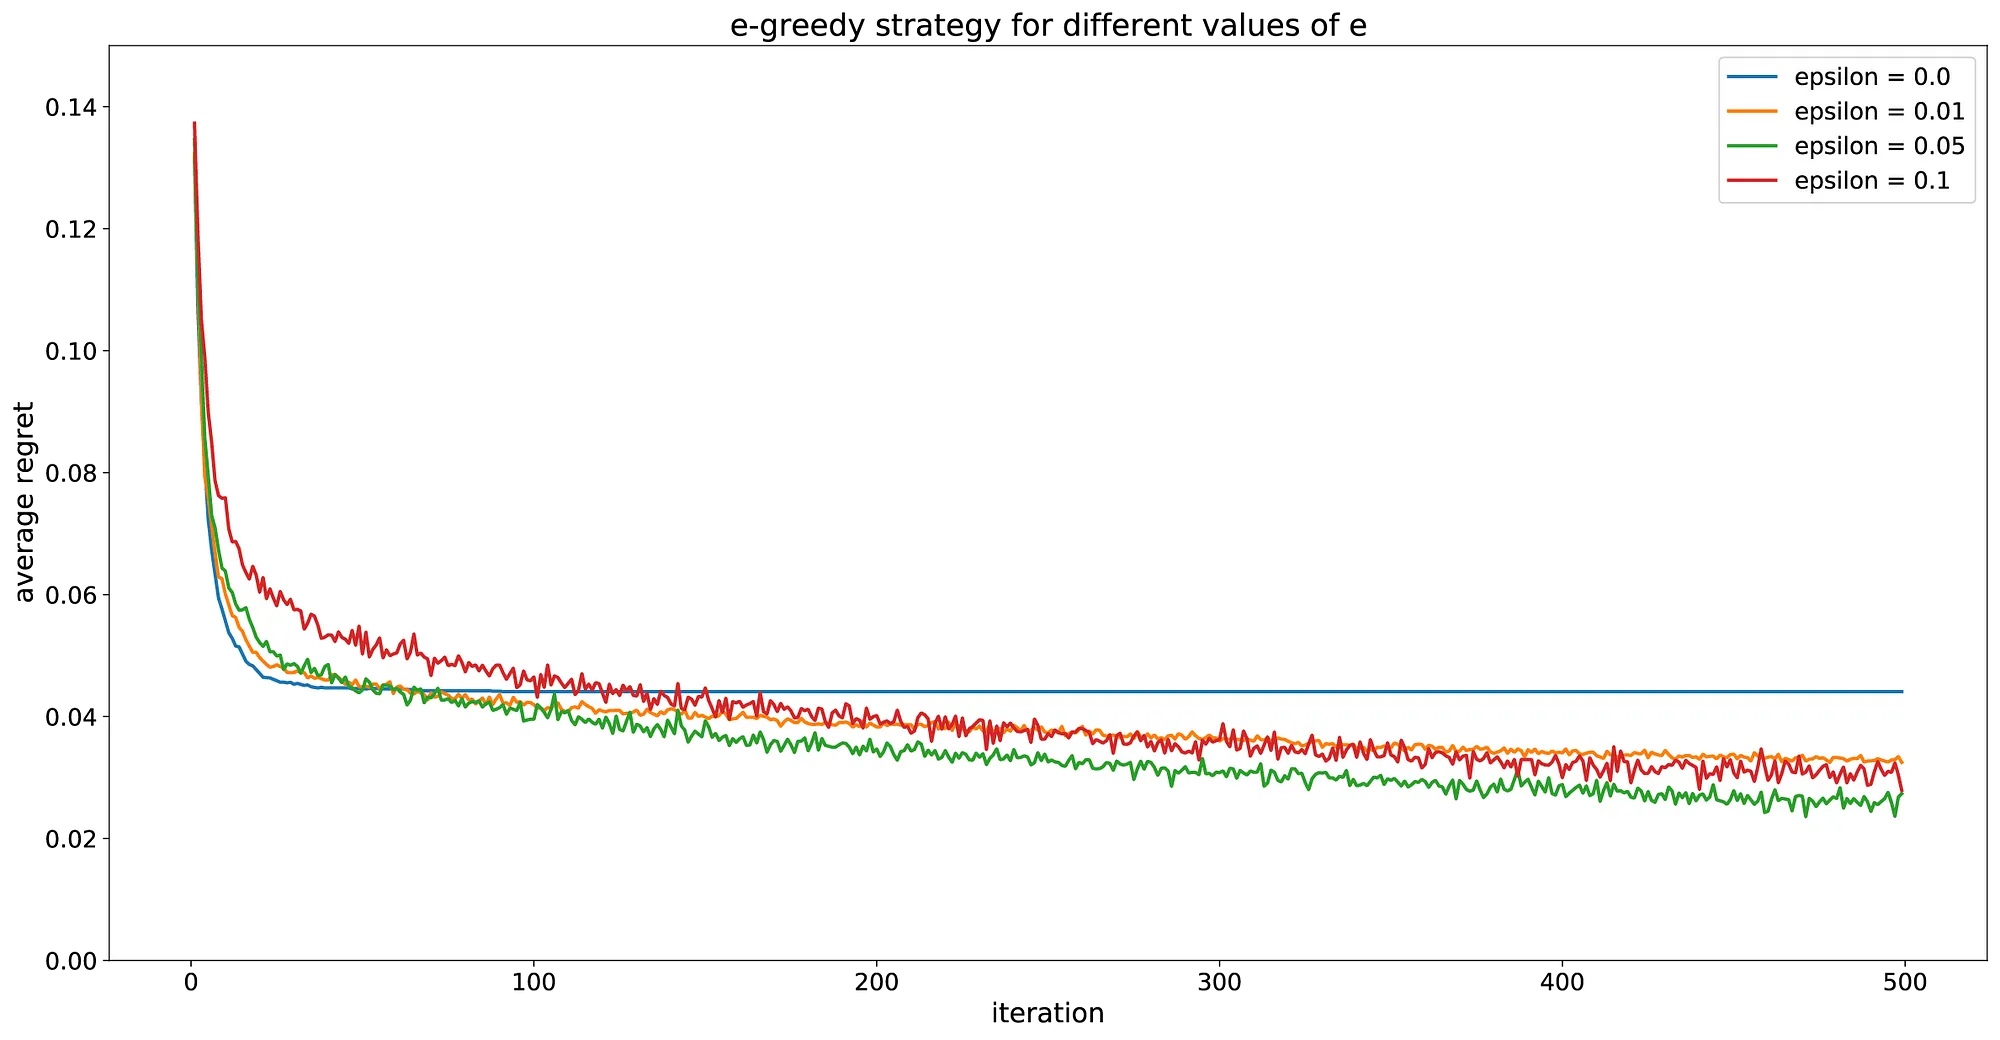
\includegraphics[width=1\linewidth]{img/results/epsilon-greedy.png}
    \caption{Average regret curves for the e-greedy strategy applied to our 3-armed bandit example with different values of epsilon.}
    \label{fig:enter-label}
\end{figure}

\subsection{Upper Confidence Bound (UCB)}

The Upper Confidence Bound (UCB) method balances exploration and exploitation by selecting actions based on their potential to yield high rewards while also considering the uncertainty of the action value estimates \cite{auer2002finite}. The UCB policy is defined as:

\begin{equation}
    \pi(a|s) = \arg\max_{a} \left( Q(s, a) + c \sqrt{\frac{\ln t}{N(s, a)}} \right)
\end{equation}

where \(t\) is the number of times the state \(s\) has been visited, \(N(s, a)\) is the number of times action \(a\) has been taken in state \(s\), and \(c\) is a constant that controls the degree of exploration.

\subsection{Boltzmann Exploration}

Boltzmann Exploration, also known as Softmax Exploration, selects actions based on a probability distribution derived from the estimated action values. The probability of selecting action (a) in state (s) is given by:

\begin{equation}
    \pi(a|s) = \frac{\exp(Q(s, a) / \tau)}{\sum_{a'} \exp(Q(s, a') / \tau)}
\end{equation}

where \(\tau\) is the temperature parameter that controls the exploration-exploitation balance. Higher \(\tau\) values lead to more exploration, while lower \(\tau\) values favor exploitation.

\subsection{Noise-Based Exploration}

Noise-Based Exploration adds random noise to the action values to encourage exploration. This method can be implemented in various ways, such as adding Gaussian noise to the action values or using Ornstein-Uhlenbeck processes for temporally correlated noise. Formally, the policy (pi) with noise \(eta\) is defined as:

\begin{equation}
    \pi(a|s) = \arg\max_{a} \left( Q(s, a) + \eta \right)
\end{equation}

\subsection{Count-Based Exploration}

Count-Based Exploration encourages visiting less frequently visited states by maintaining a count of state-action visits. Two common implementations are by hashing and by density estimation \cite{strehl2008analysis}:

\begin{itemize}
    \item \textbf{Hashing}: A hash function maps state-action pairs to a count table. The reward is augmented with a bonus that is inversely proportional to the square root of the visit count:

\begin{equation}
        R'(s, a) = R(s, a) + \frac{\beta}{\sqrt{N(s, a)}}
    \end{equation}

where beta is a hyperparameter.

    \item \textbf{Density Estimation}: This method estimates the state visitation density and uses it to guide exploration. The reward is augmented similarly to hashing, but the density is estimated using methods such as kernel density estimation.
\end{itemize}


\biblio % Needed for referencing to working when compiling individual subfiles - Do not remove
\end{document}